\documentclass{article}
\usepackage{graphicx}
\usepackage{listings}
\usepackage[dvipsnames,svgnames]{xcolor}
\usepackage{titling}
\usepackage{parskip}
\usepackage{tikz}
\usetikzlibrary{arrows.meta,positioning,shapes.geometric,fit}
\usepackage{pgfplots}
\pgfplotsset{compat=1.18}
\usepackage[
    backend=biber,
    style=apa
]{biblatex}
\usepackage[toc, nonumberlist]{glossaries}
\makeglossaries
\newglossaryentry{acid}{
    name={ACID},
    description={Atomicity, Consistency, Isolation, Durability — the four properties that guarantee database transactions are processed reliably even in the event of errors, power failures, or concurrent access}
}

\newglossaryentry{atomicity}{
    name={Atomicity},
    description={Atomicity is a fundamental database principle ensuring transactions are treated as single, indivisible "all-or-nothing" units}
}

\newglossaryentry{battlenet}{
    name={Battle.net},
    description={Blizzard Entertainment's online gaming platform and authentication infrastructure, required for connectivity in all modern Blizzard titles}
}

\newglossaryentry{btree}{
    name={B-tree},
    description={A self-balancing tree data structure that keeps data sorted and allows searches, insertions, and deletions in logarithmic time; the primary index structure used internally by SQLite}
}

\newglossaryentry{catch2}{
    name={Catch2},
    description={A header-based C++ unit testing framework that provides test case macros, assertions, and test discovery without requiring a separate test runner}
}

\newglossaryentry{cmake}{
    name={CMake},
    description={A cross-platform build system generator that produces native build files (Makefiles, Xcode projects, Visual Studio solutions) from a platform-independent description}
}

\newglossaryentry{commandlog}{
    name={command log},
    description={A durable, ordered sequence of command objects representing player actions recorded during an offline session; the primary artifact used to synchronize client state with the authoritative server on reconnection}
}

\newglossaryentry{commandpattern}{
    name={Command Pattern},
    description={A software design pattern in which each action or request is encapsulated as a self-contained object, enabling serialization, queuing, logging, and replay of operations}
}

\newglossaryentry{commutative}{
    name={commutative operation},
    description={An operation whose result is independent of the order in which it is applied relative to other operations; in this thesis, additive operations such as resource and reputation deltas that can be merged by summation}
}

\newglossaryentry{crdt}{
    name={CRDT},
    description={Conflict-free Replicated Data Type — a mathematical data structure designed so that any two replicas can be merged in any order and will converge to the same result, guaranteeing eventual consistency without coordination}
}

\newglossaryentry{dbi}{
    name={DBI},
    description={Database Interface — the abstract layer between game code and the underlying persistence backend; all state-modifying game actions are routed through the DBI, which can be swapped at runtime to target different backends}
}

\newglossaryentry{designscience}{
    name={Design Science Research},
    description={A research methodology in which the primary output is an artifact — such as an architectural design or a working software prototype — rather than an empirical study; introduced by Hevner et al.\ (2004)}
}

\newglossaryentry{entityversioning}{
    name={entity versioning},
    description={A mechanism that assigns each persistent entity a monotonically increasing version number, incremented on every committed state change; used to detect whether an entity was modified between the time a command was generated and the time it is replayed}
}

\newglossaryentry{eventsourcing}{
    name={event sourcing},
    description={A software architecture pattern in which all changes to application state are stored as an append-only sequence of events, allowing the current state to be reconstructed by replaying the event log from the beginning}
}

\newglossaryentry{idempotency}{
    name={idempotency},
    description={The property of an operation whereby applying it multiple times produces the same result as applying it once; essential for safe retry logic and duplicate detection in distributed systems}
}

\newglossaryentry{idempotencykey}{
    name={idempotency key},
    description={A unique identifier (typically a UUID) attached to each command; the server uses it to detect and silently skip commands that have already been applied, enabling safe re-transmission after network failures}
}

\newglossaryentry{Monotonically}{
    name={Monotonically},
    description={Monotonically describes a process, function, or sequence that changes in only one direction—consistently increasing or consistently decreasing without reversing direction} 
}


\newglossaryentry{mutex}{
    name={Mutex lock},
    description={In computer science, a lock or mutex (from mutual exclusion) is a synchronization primitive that prevents state from being modified or accessed by multiple threads of execution at once}
}


\newglossaryentry{noncommutative}{
    name={non-commutative operation},
    description={An operation whose result depends on the order in which it is applied; in this thesis, destructive or positional operations such as demolishing a building or placing a structure that must be validated against current server state before being accepted}
}

\newglossaryentry{occ}{
    name={OCC},
    description={Optimistic Concurrency Control — a concurrency strategy in which transactions proceed without acquiring locks, but validate that their preconditions still hold at commit time; conflicts cause the transaction to be rejected rather than blocked}
}

\newglossaryentry{orm}{
    name={ORM},
    description={Object-Relational Mapping — a layer that translates between in-memory objects and relational database rows, allowing persistent entities to be stored and retrieved without writing explicit SQL}
}

\newglossaryentry{ot}{
    name={Operational Transformation},
    description={A technique for reconciling concurrent edits by transforming operations so that they can be applied in any order while producing a consistent result; the mechanism underlying collaborative editing tools such as Google Docs}
}

\newglossaryentry{rejectionmanifest}{
    name={rejection manifest},
    description={A data structure returned to the client after a replay pass, listing each command that could not be applied along with the reason for rejection and the current server-side state of the affected entity}
}

\newglossaryentry{replay}{
    name={replay},
    description={The process of re-executing a sequence of commands against an authoritative data store in order to synchronize state; in this thesis, the mechanism by which offline commands are submitted to the server on reconnection}
}

\newglossaryentry{serverauthoritative}{
    name={server-authoritative architecture},
    description={A system design in which the server is the single source of truth for all persistent state; all state-modifying actions are validated and committed server-side, and the client cannot unilaterally alter authoritative data}
}

\newglossaryentry{servicelocator}{
    name={Service Locator},
    description={A software design pattern that provides a centralized registry through which components can obtain references to services (such as a database interface) at runtime, without being coupled to specific implementations}
}

\newglossaryentry{sqlite}{
    name={SQLite},
    description={An embedded, serverless, ACID-compliant relational database engine implemented as a C library; it stores an entire database in a single file on disk and runs within the host process, requiring no separate server}
}

\newglossaryentry{steamcloud}{
    name={Steam Cloud Save},
    description={Valve's file-level save synchronization service, which uploads and downloads save files when a player connects; conflicts are resolved by last-write-wins, discarding any changes made on the other device}
}

\newglossaryentry{telemetry}{
    name={Telemetry},
    description={Telemetry is the automated collection and transmission of data and measurements from distributed or remote sources to a central system for monitoring, analysis and resource optimization}
}

\newglossaryentry{wal}{
    name={WAL},
    description={Write-Ahead Logging — a SQLite journal mode in which changes are written to a separate log file before being applied to the main database, improving concurrent read performance and crash recovery}
}

\newglossaryentry{uuid}{
    name={UUID},
    description={Universally Unique Identifier — a 128-bit identifier standardized in RFC 4122, typically represented as a 36-character hyphen-separated hexadecimal string; used as idempotency keys to uniquely identify each command}
}

\usepackage{hyperref}

\lstset{
    basicstyle=\ttfamily\small,
    keywordstyle=\color[HTML]{0000AA}\bfseries,
    commentstyle=\color[HTML]{007700}\itshape,
    stringstyle=\color[HTML]{AA0000},
    numberstyle=\color{gray}\tiny,
    showstringspaces=false,
    breaklines=true,
    frame=single,
    rulecolor=\color{lightgray},
    backgroundcolor=\color[HTML]{F8F8F8},
}
\addbibresource{references.bib}

\title{\textbf{Bachelor thesis\\ \\Saving the Game:\\Consistent Offline-Cloud State Synchronization in Survival Video Games}\\ \\Lagre spillet:\\Konsistent synkronisering av lokal- og skybasert tilstand i overlevelsesspill\\ \\B2VISIM Bachelor in Game Technology and Simulation\\ \\SPIS2900 Bachelor thesis}
\author{\\Hans Alan Whitburn Haugen}

\begin{document}
\pagenumbering{gobble}
\begingroup

\includegraphics[width=\textwidth]{images/innlogo}
\begin{center}
\small Faculty of Audiovisual Media and Creative Technologies
\end{center}
\let\newpage\relax%
\maketitle
\endgroup
\newpage
\section*{Abstract}

Many survival games store their world entirely on remote servers. This means players cannot progress offline, and if the developer shuts down the online service, the game is lost forever. This thesis considers ways to design a system that supports both offline and online gameplay, and that allows a player to transition from an offline session to an online one without losing progress.

The main point is to log each player action in the form of a command instead of making the changes live on the server immediately. When the player is offline, the commands accumulate in a local queue. As soon as the connection is re-established, these commands are executed on the authoritative server in the same order. The biggest issue is how to reconcile conflicts: for example, if during the period of being offline, the building that a player intended to demolish was destroyed by another player, or the same territory was grabbed by another player, etc. then the system needs to figure out how to handle such situations. This thesis proposes a solution that divides commands into categories: there are commands that can always be executed irrespective of changes, some need a version check, and some still have to be rejected and communicated to the player.

A prototype was built in C++ to validate the design, including a SQLite-backed offline database and a durable command log that survives crashes.

\section*{Sammendrag}

Mange overlevelsesspill lagrer spillverdenen utelukkende på eksterne servere. Dette gjør det umulig å spille spillet offline, og hvis utvikleren legger ned nettjeneste, så mister spillerne tilgang til spillet for alltid. Denne oppgaven undersøker hvordan et system kan utvikles som gjør at en spiller kan gå mellom en spillverden uten internett og en skybasert spillverden, uten å miste fremgang.

Hovedideen er å loggføre hver spillerhandling i form av en kommando, i stedet for å gjøre endringer direkte på serveren. Når spilleren er offline, samles disse kommandoene i en lokal kø. Så snart forbindelsen er gjenopprettet, spilles de av mot den autoritative serveren i samme rekkefølge. Den største utfordringen er å avgjøre hvordan konflikter skal håndteres: for eksempel, hva skjer når annen spiller har revet ned den samme bygningen eller inntatt det samme territoriet mens en spilte frakoblet? Denne bacherloroppgaven foreslår konflikthåndteringsstrategier som klassifiserer kommandoer etter type: det er kommandoer som alltid utføres uavhengig av hva som har endret seg, andre krever en versjonssjekk, og noen må rett og slett avvises og rapporteres tilbake til spilleren.

En prototype ble bygget i C++ for å validere designet av metoden, inkludert en SQLite-basert offline database og en kommandoliste som overlever at spillet plutselig lukkes. 
\pagenumbering{roman}
\newpage

\section*{Acknowledgements}

I would like to thank my mentor, Tord Sindre Trøen, for helping me grow as a programmer and for giving me insight into the inner workings of professional game engine development and studio practices. His patience and guidance have strengthened my ability to think critically about code, particularly in the context of code reviews and the broader impact of technical changes. He also introduced me to effective ways of using AI to support code production, while maintaining a critical perspective on the generated results. In addition, he emphasized the importance of seeking help when needed and reaching out to others with prior experience in the systems I work with — advice that has reinforced similar guidance I have received from mentors in the past.

I would also like to thank Maria Esperanza Johnson Ruiz for her continued support throughout the course. I am grateful to Andreas Aasom Brandsnes, who has been an excellent collaborator and a kind friend on past projects. I would further like to thank Håvard Vibeto at the University of Inland Norway, Fredrik Martol at Funcom, and the Funcom Core Engine Team for giving me the opportunity to experience game development within a cutting-edge studio environment.

I would also like to thank my academic advisor at the University of Inland Norway, Ole Einar Flaten, who teaches 3D programming and game engine development—two of my primary areas of interest. His feedback and academic guidance have been invaluable throughout the thesis process, as well as during the internship period from 15 January to 13 May 2026.

AI has been used to help drafting prose, structuring arguments, and assisting with the implementation. Design decisions, benchmark data, and conclusions are my own.

\newpage

\tableofcontents{}

\newpage

\lstlistoflistings

\newpage

\pagenumbering{arabic}

\section{Introduction}

This investigation considers a way to develop the persistence system of a modern large-scale survival multiplayer game. The design targets persistent multiplayer worlds shared by thousands of players, and are intended to support the storage of player progression, world state, and faction dynamics. The design is not concerned with ephemeral information such as player position or real-time combat replication; the focus is on long-term persistent data of the kind typically stored in centralized, cloud-hosted SQL databases.

The suggested design is intended to provide a way to support both offline and online functionality. Having the ability to make a game run offline is important, especially on console platforms where access to online multiplayer features typically requires a paid subscription service. A significant portion of console players therefore do not participate in online multiplayer environments \autocite{onlinegamers}. Playing with friends should be supported via local cooperative modes, both splitscreen and local listen server setup, while preserving core gameplay mechanics.

This requirement introduces architectural challenges which need to be addressed sensibly. Games on the market which support persistent game state stored exclusively in cloud-based SQL databases assume continuous server connectivity. Supporting offline gameplay necessitates a hybrid architecture in which persistent world state can be stored locally, potentially using embedded database solutions such as SQLite which can later be synchronized with the authoritative cloud-based server infrastructure.

Many gamers prefer to play offline, but might want to connect online as they advance in the persistent world. Collaboration with other players is often necessary in survival games to navigate the harsh environment. Political dynamics and faction-based conflict play a central role in survival games, as groups of players compete for control and influence within the game’s persistent world \autocite{CERE2021105}. Designs that allow users to transition online after initial offline sessions are explored.

The following research statement is investigated:

\subsection*{How can an offline-online synchronization system for game persistence targeting survival multiplayer games be designed and evaluated with respect to consistency, conflict resolution, and reconnection performance?}

\newpage

\section{Methodology}

A design science research approach \autocite{hevner2004design} has been adopted. In Design Science, the main product of the thesis is an artifact; in this project the artifacts are the architectural design of a save system and the actual implemented software prototype of the artifact. Instead of the empirical study, the software prototype is the main end product of the research.

The research is conducted in three phases. The first stage is analysis: it involves analyzing existing, server authoritative persistence systems and identifying the problems associated with playing offline. This analysis is performed in Section~\ref{sec:challenges}.

Proposal for second stage design: a hybrid architecture derived from the Command Pattern, with conflict resolution, and showing how the design fits together with online SQL backends and a local SQLite store, is proposed. Design decisions are recorded in Section~\ref{sec:architecture}.

The third stage is evaluation, implemented in C++, against two requirements:

\begin{enumerate}
\item Correctness, where all parts of the design are covered by automated unit and integration tests, written using the Catch2 framework \autocite{catch2}. 
\item Performance, where the replay throughput, command log size limits, conflict detection overhead, and the end-to-end cost of a full offline session are measured using a suite of benchmark programs.
\end{enumerate}

Alternative solutions to the research question are briefly discussed in Section~\ref{sec:alt}. The evaluation is described further in Section~\ref{sec:evaluation}. The results are discussed in Section~\ref{sec:discussion} and future work is touched upon in Section~\ref{sec:futurework}. Finally, a conclusion is made in Section~\ref{sec:conclusion}.

\newpage

\section{Related Work}
\label{sec:relatedwork}

\subsection{Game Industry Approaches}

Several games available on the market have tried to solve the problem of syncing game data between playing offline and online. The game's developers do not typically disclose how they do it.

Valheim \autocite{valheim} uses SQLite to store its world state locally on player's machines. The entire saved game is found in \texttt{world.db}. SQLite makes the game fully playable offline. However, if two players host separate copies of the same world while disconnected, there is no supported way to rejoin and merge the database differences. This is the snapshot problem described in Section~\ref{sec:challenges}. SQLite makes it straightforward to implement single-player sessions but rejoining an online session with SQLite introduces challenges regarding cheating and consistency.

Steam Cloud Save \autocite{steamcloud} enables folders and files to be synchronized between computers by hosting them on Valve's servers. The save data is uploaded and downloaded when players connect to Steam. Conflicts are resolved by making the most recently modified file the one which is stored on the server, a last-write-wins system. This approach is simple and adequate for single-player games, but cannot handle merging modifications from multiple players.

World of Warcraft \autocite{wow} is one of the earliest examples of a MMO which is based on the server-authoritative model. All of the persistant game state is stored on Blizzard's servers. All items, character properties, quests and guild information is stored remotely. When Blizzard stopped the legacy vanilla servers in 2016, all the game data, the characters, player progression, everything done in the game world was lost, which is another example of the preservation problem discussed in Section~\ref{sec:discussion}.

Blizzard Entertainment's Diablo III \autocite{diablo3} required online connectivity to the Battle.net service even for solo gameplay, their new game required all character state to be stored and validated server-side. At launch in 2012 server overload made the game completely unplayable despite no multiplayer interaction being involved. This is widely referred to as "Error 37" and illustrates how the purely server-authoritative model can fail. If the game depends entirely on the availability of the developer's infrastructure, regardless of whether the player is interacting with others, the game becomes unplayable if the developers have server problems.

Many large-scale survival multiplayer games, such as Rust and DayZ, take the same approach. Offline play becomes impossible, requiring a constant internet connection to a central server. This sidesteps offline to online persistence synchronization entirely, but at the cost of offline-mode.

Academic distributed systems literature has studied the problem and offers solutions, though they are often overly complex:

Conflict-free Replicated Data Types (CRDTs) \autocite{shapiro2011crdts} are data structures that can be replicated over several computers and can be changed immediately with a guarantee of eventual consistency with the other computers. Any two replicas can be merged out of order but will eventually give the same result on all computers. CRDTs would eliminate the need for conflict resolution policies entirely. However, the entire game would need to be redesigned. Every data type would have to adhere to CRDT semantics. This is a significant architectural investment. They are also better suited to data types like counters and sets than to the complex relational structures (buildings with positions, quest state, faction information, map markers) that survival games require.

Operational Transformation (OT) \autocite{ellis1989ot}, the technique underlying WYSIWfS (what you see is what I see) editing tools such as Google Docs, transforms operations so that they can be applied out of order and still produce the same document. The intent-based approach is similar to the model in this thesis, commandlog shares similarities with OT. The command-based approach and OT both consider operations rather than snapshots. However, OT requires a central server to sequence and transform operations in real time. This is not possible during an offline play session.

Event sourcing \autocite{fowler2005eventsourcing} is a software architecture pattern where the program state is constructed by unwinding an append-only log of events. The command log proposed in this thesis is very similar to this architecture: both record intent rather than state and both allow the current state to be reconstructed by replaying the log. The main difference is that event sourcing assumes a single authoritative log, whereas this thesis addresses what happens when two divergent logs (client offline, server online) must be merged.

The conflict resolution strategy, which uses entity versioning and optimistic concurrency control, follows the approach described by Bernstein and Goodman \autocite{bernstein1981concurrency}. Here, transactions validate the legality of actions at commit time rather than acquiring locks upfront. It is typical to make data consistent by relying on mutexes: a thread or process is given an exclusive lock before modifying shared state, blocking all other writes until the lock is released. This works well when everyone is continuously connected to an online server, but for offline sessions holding a lock while disconnected would stall the entire system. Optimistic concurrency control solves this by allowing offline progress to proceed freely and doing conflict detection when users reconnect to the server. This is why the conflict resolution from Bernstein and Goodman becomes a natural fit for the Command-based offline–online model presented in this thesis.

Kleppmann et al.\ \autocite{kleppmann2019local} calls software which should work offline a \emph{local-first} software problem: applications should keep data locally, not on the cloud, and remain fully functional without a network connection. Synchronization with collaborators or cloud services should only occur when the user is ready and connects online. The command log approach proposed in this thesis is a \emph{local-first} problem designed to be compatible with survival multiplayer games. The commandlog operates on persistent state that is shared by many players. In the model presented in this thesis, an authoritative server must eventually become the final source of truth.

Moll et al. \autocite{MOLL2021107723} present a quadtree-based protocol to sync game state across server clusters, so called Named Data Networking. While they focus on inter-server sync rather than offline play, they show that region-based naming and decoupled representations can cut the overhead of keeping distributed states consistent. A concern related to the scalability dimension of the problem addressed later in the thesis in Section~\ref{sec:scale}.

\newpage

\section{Typical Challenges in Persistence Systems}
\label{sec:challenges}

Game worlds consist of actors that may own inventory items, buildings, vehicles, navigation markers, abilities, and quest progression. In large-scale online survival games, persistent game state is commonly stored in centralized persistence systems backed by SQL databases hosted on cloud infrastructure.

Such systems typically follow a server-authoritative architecture in which all state-modifying actions are processed through a centralized backend. Player actions are buffered temporarily on the client before being committed to the authoritative server. Multiple server instances may run concurrently, but at any given time only one instance holds authoritative control over a given player or region. Actions are executed as database transactions, providing rollback in the event of failure.

A common design pattern for this kind of system is to apply the Service Locator pattern \autocite{nystrom2014servicelocator} to abstract the communication layer responsible for generating and dispatching persistence commands. This abstraction is hereafter referred to as the Database Interface (DBI). Rather than issuing raw SQL queries directly from game code, the DBI invokes predefined server-side functions. Each function executes as a transactional unit and can be rolled back if any step fails, so every state-modifying action is encapsulated as an atomic database operation.

A well-designed DBI supports atomicity, consistency, and \gls{idempotency}. If a network failure occurs, or if the client is uncertain whether a transaction completed, the DBI can safely retry without risking duplicate or inconsistent state changes. An important structural advantage of this abstraction is that the DBI can be swapped out via the Service Locator pattern: an online session routes calls to the remote SQL backend, while an offline session could route them to a local implementation — the implications of which are explored in Section~\ref{sec:architecture}.

A SQL-based DBI architecture treats the cloud-hosted SQL database as the single authoritative source of truth for all persistent game state. This provides strong consistency guarantees in fully online environments, but it inherently depends on centralized authority and does not account for state divergence in disconnected scenarios. See the listing below:

\newpage

\begin{lstlisting}[language=C++, caption={DBI interface (abstract base class)}]
class IDatabaseInterface
{
public:
    virtual ~IDatabaseInterface() = default;

    virtual bool CreateBuilding(int32_t playerId, int32_t buildingTypeId,
                                float posX, float posY, float posZ) = 0;
    virtual bool DestroyBuilding(int32_t buildingId) = 0;

    virtual bool TransferItem(int32_t fromPlayerId, int32_t toPlayerId,
                              int32_t itemId, int32_t quantity) = 0;

    virtual bool CompleteQuest(int32_t playerId, int32_t questId) = 0;

    virtual bool UpdateFactionRelation(int32_t factionA, int32_t factionB,
                                       int32_t relationDelta) = 0;
};
\end{lstlisting}

\subsection{Limitations of Server-Authoritative Architectures}

A server-authoritative persistence architecture requires continuous internet connectivity to a centralized cloud-based server. Although this model is good for consistency, all players in online game will without question see the same data and be in the same world, it entails significant drawbacks when developers want to support offline or hybrid offline-online game modes:

Since all actions that will change the database data are executed as remote transactions, gameplay cannot progress without server access. This makes offline play impossible. If the online service is shut down, the game will no longer function. It also becomes more difficult to deploy the game on platforms where online access requires a paid subscription. If a player loses internet connectivity mid-session, for example due to server maintenance, gameplay cannot continue. The client has no way to queue actions for later submission. For players from regions with unreliable internet connectivity, the game becomes more or less inaccessible. The combined architecture described in Section~\ref{sec:architecture} tackles these limitations by decoupling action generation from action transmission.

In a purely server-authoritative model, the client does have a local database of the world state. While a temporary state may exist in memory during a session before being transmitted to an online server, durable storage is managed exclusively by remote infrastructure. This prevents local world progression during disconnection and support for local cooperative play modes becomes difficult to implement. Implementing a local persistence layer, such as the SQLite-backed DBI described in Section~\ref{sec:sqliteimp}, enables progress to persist across by writing state to disk which will allow offline sessions.

A server-authoritative architecture expects all state changes to happen linearly and does not allow modifications from offline sessions. For example, both offline players and the live server may modify the same entity independently. As a result, such architectures usually lack:

\begin{enumerate}
  \item \textbf{Entity version tracking}: Without having a way to know which version of an entity a player has acted on, it is impossible to determine whether the action has happened on outdated information.
  \item \textbf{Conflict identification}: Without entity version tracking it is not possible to detect conflicts which occur when two or more players modify the same entity in conflicting ways.
  \item \textbf{Deterministic merging}: When a conflict has been detected, conflict resolution must take place. An authorative server typically has no rules for such an action when all actions happen in transactions: last-write-wins, action rejection, or type-specific merging can be implemented to support offline sessions.
\end{enumerate}

Without the above points, synchronization of locally modified state with cloud-based state is not possible. The version-based conflict recognition and command classification strategy described in Section~\ref{sec:conflictresolution} addresses all three gaps.

\newpage

\section{Proposed Hybrid Persistence Architecture}
\label{sec:architecture}

\subsection{Command-Based State Replication}
\label{sec:commandbased}

To enable offline progression without completely redesigning the server-authoritative model, this thesis proposes a command-based persistence model inspired by the Command Pattern as originally described in Design Patterns: Elements of Reusable Object-Oriented Software \autocite{gamma1994design} and presented specifically for games development in Game Programming Patterns \autocite{nystrom2014game}.

Rather than directly transmitting changes to the cloud-based database, during offline sessions the player actions are encapsulated as serializable command objects. Each command represents an intention instead of just a state change. An action is for example to create a building, transfer an item, complete a quest or place map marker. A command will also have parameters which allows the server to convert the command into a SQL modification which can be executed on the server when the player reconnects online.

In other words, during an offline session commands are appended to a local command log. The commands are not transmitted immediately to the server. When connectivity is restored, the queued commands are transmitted sequentially to the authoritative backend cloud-server and executed as transactional operations.

This approach introduces several advantages:

\begin{enumerate}
  \item Commands are easy to serializable and can be stored locally.
  \item Replaying commands enables deterministic reconstruction of state.
  \item The command log provides a history of offline actions.
  \item The server-side transaction logic does not need to change at all.
  \item Fraud detection can rely on the old system.
\end{enumerate}

By storing intent rather than state, the game will not diff to databases and merge them but instead achieves synchronization by executing state-modifying operations in order. See the listing below:

\newpage

\begin{lstlisting}[language=C++, caption={Command structure and local command log}]
struct Command
{
    std::string type;            // e.g. "CreateBuilding", "AddMoney"
    int64_t     timestamp;       // UTC milliseconds at time of action
    std::string idempotencyKey;  // UUID to detect duplicate replays
    std::string entityId;        // ID of the affected entity
    int32_t     expectedVersion; // entity version at command creation
    int32_t     delta;           // delta for commutative operations
};

class CommandLog
{
public:
    void                 Append(const Command& cmd);
    std::vector<Command> GetPending() const;
    void                 MarkFlushed(const std::string& idempotencyKey);
    void                 MarkFlushedBatch(
                             const std::vector<std::string>& keys);
    std::size_t          PendingCount() const;

private:
    std::vector<Command> m_pending;
};
\end{lstlisting}

\subsection{Implementation considerations}

Security considerations are important when dealing with online games, it is important to make sure players do not cheat and create false information. This system must be designed to be secure. The suggested system allows commands to be generated client-side and stored locally. A malicious client could potentially create or alter commands and add them to the local queue before transmission to the server. Every command must therefore be validated server-side before a transaction is committed, and any command that produces an invalid or impossible state transition must be rejected. Conflict detection, entity versioning, and per-type resolution policies are addressed in the following subsection.

Two other concerns need to be addressed as well. The first one is ordering guarantees: the command log must always represent a sequence of commands in in the order they were taken while offline. The server must replay them in that order to ensure deterministic results. Second, idempotency. If the same command is added twice, which could happen due to bugs in the gameplay code or unexpected player behaviour, or if the execution of a command fails, the server must be able recover and skip said commands. The idempotency key found in the command-struct (see listing above) serves this purpose.

Lastly, what should the server do if commands depend on entities which have been removed on the server-side? If an offline command expects an entity to exist which has been deleted by another player during an online session, the commands will no longer make sense. Handling this requires more than simple version-checks, the game will need to be able to provide a rejection manifest of items or structures which could not be applied to the online database due to divergence in the online game state of the game world.

\subsection{Conflict Resolution Strategy}
\label{sec:conflictresolution}

When offline commands are replayed against the authoritative server, conflicts can arise. When the server state diverges from the state the offline player world state, the commands generated might need to be rejected. As the game world evolves and diverges online, commands generated during offline sessions could become invalid or inconsistent with the state on the server and will not transition to the online server during a reconnection online. Ways to handle this are explored next:

\subsubsection{Conflict Detection via Entity Versioning}

Each persistent entity in the database (inventory item slot, map marker, quest, building, etc.) is assigned an ever-increasing version number. This is called a monotonically incremented number which increases with every committed state change. This is the expectedVersion field in the listing above. When a command is generated offline, it will look into the local database for the version of the entity the player has manipulated and add it to the command. When the player reconnects and the commands are replayed, the server will compare the recorded version against the current entity version. The online version number will increase and go out of sync with the offline version number if other players have manipulated the same object, and conflict resolution can take place, for example the command can be rejected.

This is very similar to Optimistic Concurrency Control (OCC) which is used in traditional database systems. Transactions proceed without locking but are validated at commit time \autocite{bernstein1981concurrency}.

\subsubsection{Command Classification}

Just because entity versions do not match between local and server sessions, the command does not necessarily need to be rejected. Commands have different types and different conflict resolution strategies:

\begin{enumerate}
  \item \textbf{Idempotent commands} — Quest completion, achievement unlocks, and similar boolean flags. These produce the same result regardless of how many times they are applied and can be safely replayed without harm.
  \item \textbf{Commutative commands} — Additive operations such as resource collection, experience points, or money deltas. The order does not change the final value. These commands can simply have their deltas summed together with the existing entity.
  \item \textbf{Non-commutative commands} — Spatial operations or building related such as destroying a building or placement of a vehicle. These need to be rejected and communicated to the reconnecting player if there is a conflict with server entities.
\end{enumerate}

\subsubsection{Resolution Policies}

For each conflict type a deterministic resolution must take place on the server before the command is committed. See listing below:

\begin{lstlisting}[language=C++, caption={Server-side command validation and conflict resolution}]
ReplayResult ReplayCommand(const Command& cmd, Database& db,
                           RejectionManifest& manifest)
{
    // Idempotent: already applied, skip silently
    if (db.IsAlreadyApplied(cmd.idempotencyKey))
        return ReplayResult::Duplicate;

    // Commutative: apply delta regardless of entity version
    if (cmd.type == "MoneyDelta")
        return db.ApplyDelta(cmd);

    // Non-commutative: validate entity state before committing
    Entity entity = db.GetEntity(cmd.entityId);

    if (!entity.exists)
    {
        manifest.push_back({cmd, ReplayResult::Rejected});
        return ReplayResult::Rejected;
    }

    if (entity.version != cmd.expectedVersion)
    {
        manifest.push_back({cmd, ReplayResult::Conflict});
        return ReplayResult::Conflict;
    }

    return db.Commit(cmd);
}
\end{lstlisting}

\subsubsection{Rejection Manifest}

Commands that fail validation are not silently discarded. Instead, they are collected into a rejection manifest that is returned to the client after the replay pass completes. The manifest records the command type, the reason for rejection, and the current server-side state of the affected entity. This allows the game to inform the player of which offline actions could not be applied and why, enabling the client to present meaningful feedback rather than silently losing progress.

\subsection{Command Dispatch and SQL Execution}
\label{sec:dispatch}

Once \texttt{ReplayCommand} determines that a command passes validation, it calls \texttt{db.Commit(cmd)}. The commit step dispatches on the command's \texttt{type} field and invokes the corresponding method on the DBI, which translates the operation into one or more SQL statements. The mapping is straightforward: each command type corresponds directly to a single DBI method, and each DBI method is responsible for the SQL that implements the game-domain operation it represents.

\begin{lstlisting}[language=C++, caption={Server-side command dispatch to DBI methods}]
ReplayResult Database::Commit(const Command& cmd)
{
    if (cmd.type == "CreateBuilding")
        dbi.CreateBuilding(cmd.entityId, cmd.delta, 0, 0, 0);
    else if (cmd.type == "DestroyBuilding")
        dbi.DestroyBuilding(cmd.entityId);
    else if (cmd.type == "TransferItem")
        dbi.TransferItem(cmd.entityId, cmd.delta);
    else if (cmd.type == "CompleteQuest")
        dbi.CompleteQuest(cmd.entityId, cmd.delta);
    else if (cmd.type == "ResourceDelta" ||
             cmd.type == "ReputationDelta")
        dbi.UpdateFactionRelation(cmd.entityId, cmd.delta);

    RecordApplied(cmd.idempotencyKey);
    IncrementVersion(cmd.entityId);
    return ReplayResult::Committed;
}
\end{lstlisting}

Each DBI method executes a specific SQL pattern chosen to preserve the correctness properties of that command class:

\begin{center}
\begin{tabular}{lll}
\hline
Command type & DBI method & SQL pattern \\
\hline
\texttt{CreateBuilding}  & \texttt{CreateBuilding}        & \texttt{INSERT INTO buildings} \\
\texttt{DestroyBuilding} & \texttt{DestroyBuilding}       & \texttt{DELETE FROM buildings WHERE id = ?} \\
\texttt{TransferItem}    & \texttt{TransferItem}          & \texttt{BEGIN; SELECT / UPDATE / UPSERT; COMMIT} \\
\texttt{CompleteQuest}   & \texttt{CompleteQuest}         & \texttt{INSERT OR IGNORE INTO completed\_quests} \\
\texttt{ResourceDelta}   & \texttt{UpdateFactionRelation} & \texttt{INSERT … ON CONFLICT DO UPDATE SET} \\
\texttt{ReputationDelta} & \texttt{UpdateFactionRelation} & \texttt{relation = relation + excluded.relation} \\
\hline
\end{tabular}
\end{center}

The SQL patterns are not arbitrary. \texttt{INSERT OR IGNORE} for quest completion makes the operation inherently idempotent at the database level — a duplicate replay of the same quest completion is silently discarded even if the idempotency check at the application level somehow fails. The UPSERT pattern for resource and reputation deltas (\texttt{ON CONFLICT DO UPDATE SET value = value + excluded.value}) accumulates the delta additively, which is the correct merge behaviour for commutative operations regardless of how many times the command is replayed. The explicit \texttt{BEGIN}/\texttt{COMMIT} transaction wrapping \texttt{TransferItem} ensures that the debit from the sender and the credit to the recipient are atomic — either both succeed or neither does, preventing inventory from being created or destroyed by a partial failure.

\subsection{Integration Possibilities}

In a server-authoritative game, every action that should persist goes through the DBI. By extending the DBI into a factory that produces command objects, the system can route actions in two ways depending on connectivity state: online commands are transmitted to the server immediately, while offline commands are serialized and stored on disk, deferred until the player reconnects.

The routing decision is straightforward to implement. A factory function checks connectivity and returns the appropriate DBI implementation:

\begin{lstlisting}[language=C++, caption={Connectivity-aware DBI factory}]
std::unique_ptr<IDatabaseInterface> CreateDBI(bool isOnline)
{
    if (isOnline)
        return std::make_unique<RemoteSQLDBI>(serverConfig);
    else
        return std::make_unique<SQLiteDBI>("offline.db");
}
\end{lstlisting}

Game code calls DBI methods without knowing which backend is active. When connectivity is restored, the engine drains the durable command log by calling \texttt{ReplayAll}, which submits each queued command to the server in order and returns a \texttt{RejectionManifest} listing any commands that could not be applied.

Figure~\ref{fig:architecture} shows the overall data flow.

\begin{figure}[h]
\flushleft
\resizebox{\linewidth}{!}{%
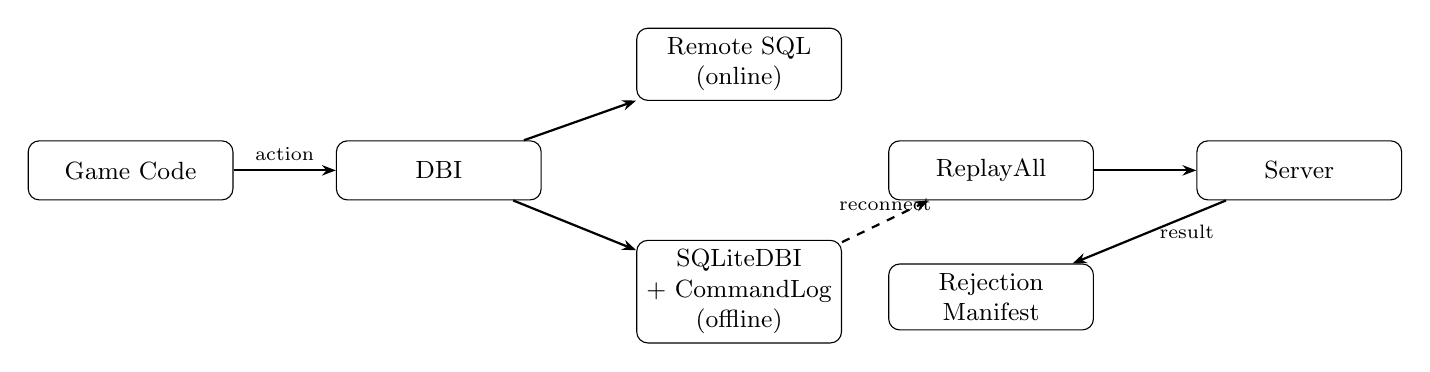
\begin{tikzpicture}[
    node distance=0.9cm and 1.3cm,
    box/.style={draw, rounded corners, minimum width=2.6cm, minimum height=0.75cm,
                align=center, font=\small},
    arr/.style={-{Stealth[length=5pt]}, thick},
    dasharr/.style={-{Stealth[length=5pt]}, thick, dashed}
]
    \node[box] (game)   {Game Code};
    \node[box, right=of game] (dbi) {DBI};
    \node[box, above right=0.5cm and 1.2cm of dbi] (remote) {Remote SQL\\(online)};
    \node[box, below right=0.5cm and 1.2cm of dbi] (sqlite) {SQLiteDBI\\+ CommandLog\\(offline)};
    \node[box, right=4.4cm of dbi] (replay) {ReplayAll};
    \node[box, right=of replay] (server) {Server};
    \node[box, below=0.8cm of replay] (manifest) {Rejection\\Manifest};

    \draw[arr]    (game)   -- node[above,font=\scriptsize]{action} (dbi);
    \draw[arr]    (dbi)    -- (remote);
    \draw[arr]    (dbi)    -- (sqlite);
    \draw[dasharr](sqlite) -- node[above,font=\scriptsize]{reconnect} (replay);
    \draw[arr]    (replay) -- (server);
    \draw[arr]    (server) -- node[right,font=\scriptsize]{result} (manifest);
\end{tikzpicture}%
}
\caption{Hybrid persistence architecture: game code interacts only with the DBI; the active implementation is swapped at runtime depending on connectivity.}
\label{fig:architecture}
\end{figure}

\subsection{Prototype Implementation}

A self-contained C++ prototype of the proposed architecture was developed alongside this thesis and is available at:

\begin{center}
\url{https://github.com/alanhaugen/SPIS2900-Bachelor}
\end{center}

The prototype is located in the \texttt{app/} directory and is built with CMake. It depends only on Catch2, which is fetched automatically at configure time, and a system SQLite3 library. The implementation is organized as two libraries:

\textbf{\texttt{offline\_sync\_lib}} contains the core persistence abstractions:
\begin{itemize}
  \item \texttt{IDatabaseInterface} — the abstract DBI used by game code, with virtual methods for all persistent game actions.
  \item \texttt{Command} and \texttt{CommandLog} — the in-memory command queue described in Section~\ref{sec:commandbased}.
  \item \texttt{Database} — a lightweight in-memory entity store used for testing, with version tracking and idempotency key recording.
  \item \texttt{ReplayCommand} / \texttt{ReplayAll} — the conflict-resolution algorithm from Section~\ref{sec:conflictresolution}, including the \texttt{RejectionManifest} type.
\end{itemize}

\textbf{\texttt{offline\_sync\_sqlite\_lib}} contains the SQLite-backed implementations:
\begin{itemize}
  \item \texttt{SQLiteDBI} — a concrete implementation of \texttt{IDatabaseInterface} that stores game state in a local SQLite file. It maintains game-domain tables for buildings, item inventories, completed quests, and faction relations. Item transfers execute inside an explicit SQLite transaction and are rejected atomically if the sender has insufficient inventory. Quest completion uses \texttt{INSERT OR IGNORE} to preserve idempotency. Faction relation updates use an UPSERT to accumulate signed deltas.
  \item \texttt{SQLiteCommandLog} — a durable replacement for the in-memory \texttt{CommandLog} that writes each command to a SQLite file before returning. The \texttt{idempotency\_key} column carries a \texttt{UNIQUE} constraint so that a double-append is silently discarded at the database level. Commands survive process restarts and can be recovered on next open.
\end{itemize}

The prototype includes 31 Catch2 unit tests covering the command log, idempotency, commutative merging, non-commutative conflict detection, SQLite persistence, and a full offline-session integration scenario.

\newpage

\section{Alternative State Replication Persistence Architectures}
\label{sec:alt}

Other simpler alternatives to the Command-Based State Replication have been considered and will be described and discussed below. Some of the problems with the alternative architectures revolve around a lack of functionality for solving divergent state (see section \ref{sec:sqliteimp}) and implementation complexity (see section \ref{sec:ormimp}).

\subsection{Local Persistence via SQLite}
\label{sec:sqliteimp}

A direct approach to enabling offline functionality is to extend the Database Interface (DBI) abstraction with a complete SQLite-backed implementation. Rather than communicating with remote SQL servers, the DBI would execute equivalent operations against a locally embedded SQLite database during offline sessions.

SQLite \autocite{sqliteorg} is an embedded, serverless, ACID-compliant relational database engine that operates as a lightweight C/C++ library. Unlike other SQL implementations, it does not require a separate server process; instead, it runs within the host application and stores data in a single file on disk. This makes it well-suited for offline persistence in desktop and console environments.

By preserving the DBI abstraction layer, the system can maintain a consistent programming interface for persistence operations regardless of connectivity state. When offline, DBI calls would be routed to the SQLite backend. When online, calls would be directed to the existing SQL infrastructure.

This design minimizes disruption to the gameplay code, as the persistence boundary remains unchanged. However, it introduces challenges related to schema compatibility, transaction semantics, and synchronization between the local SQLite instance and the authoritative cloud database.

A deeper limitation is that a SQLite-backed DBI alone is not sufficient for synchronization. The SQLite DBI is a \emph{readable state store} — it answers the question "what does the world look like right now?" and allows the game to display inventory, buildings, and quest progress during an offline session. What it does not provide is a record of what \emph{changed} during that session. On reconnection, the server has no way to know which operations the player performed; it can only observe that local and remote state have diverged. Merging two divergent snapshots requires structural diffing of every entity, which becomes increasingly error-prone as the world model grows more complex.

A structural diff is insufficient for two deeper reasons. First, a diff records \emph{what changed}, not \emph{what the player did}: if a player's gold balance fell by 20, the diff sees $-20$, but whether that was a purchase, a trade, or a quest cost determines which server-side validation rules apply and what happens if the change is rejected. Without the originating operation, the server cannot classify the change or apply a meaningful resolution policy. Second, operations that cancel within a session leave no trace: if a player builds a structure and then demolishes it while offline, the net diff is empty — yet both actions consumed resources and triggered side-effects that the server must account for. A command log captures every step; a diff only captures the outcome.

This is why the command log is a necessary complement rather than an optional addition. The command log is a \emph{pending change queue} — it records each action as it is taken so that the exact sequence of player intent can be replayed on the server. After a successful replay the log is drained; the SQLite state store is not. The two components answer different questions and cannot substitute for each other: removing the command log leaves no replay record, while removing the SQLite DBI leaves the game unable to read any state while offline.

\subsection{ORM (Object-Relational Mapping)}
\label{sec:ormimp}

An alternative architectural approach considered was the introduction of an Object–Relational Mapping (ORM) system. An ORM provides a layer that maps in-memory C++ objects directly to relational database structures, allowing persistent entities to be stored and retrieved without writing explicit SQL logic. In such a system, game objects (e.g., inventory items, buildings, or quests) would be automatically translated into database rows and reconstructed from relational data.

ORM frameworks are common in higher-level languages such as Python and Java, where reflection and dynamic typing simplify runtime type inspection and schema generation. In contrast, implementing a fully featured ORM in C++ presents additional complexity due to the lack of built-in reflection and the need for explicit type registration and serialization logic.

The deeper problem, however, is a fundamental mismatch between the ORM model and the command-based architecture proposed in this thesis. An ORM operates on \emph{state}: it tracks which object fields have changed and generates SQL to persist the new snapshot. The command log operates on \emph{operations}: it records what the player did, not what the resulting world state looks like. These two models are philosophically opposed. If an ORM were used as the persistence layer, it would continuously collapse player actions into state diffs, discarding precisely the operation-level intent that the command log needs to preserve for server-side replay. The server would receive a snapshot of what changed, not a replayable record of how it changed — making conflict classification by command type impossible.

By contrast, the DBI abstraction already provides the backend-agnosticism that an ORM is typically chosen for: game code interacts with a stable interface and is unaware of whether calls are routed to a remote SQL server or a local SQLite file. The difference is that the DBI exposes game-domain operations (\texttt{TransferItem}, \texttt{CompleteQuest}) rather than generic object persistence, which is exactly the granularity needed to classify commands for conflict resolution. The DBI is, in effect, a domain-specific alternative to a generic ORM — and for this use case, the domain-specific design is the more appropriate choice.

\newpage

\section{Evaluation}
\label{sec:evaluation}

The prototype was evaluated along two dimensions: correctness, verified through automated testing, and performance, measured through a benchmark suite run on the same hardware used for development (Apple M-series, macOS, Release build with compiler optimisations enabled).

\subsection{Correctness}

The implementation is covered by 31 Catch2 unit and integration tests organised into five categories: command log behaviour (append, ordering, flush), idempotency (duplicate commands produce no side effects), commutative merging (resource and reputation deltas apply regardless of version mismatch), non-commutative conflict detection (version mismatch and missing entities are caught and reported), and a full offline session integration test that exercises all result types in a single replay pass. All 31 tests pass.

\subsection{Replay Throughput}

The first benchmark measures how quickly the in-memory replay engine can process a command log of increasing size, using one unique entity per command to isolate the cost of the replay loop itself from conflict resolution overhead.

\begin{center}
\begin{tabular}{rrrr}
\hline
Commands & Time (ms) & Throughput (cmd/s) & Applied \\
\hline
100      & 0.02      & 4,907,975          & 72      \\
500      & 0.09      & 5,780,347          & 368     \\
1,000    & 0.16      & 6,448,160          & 734     \\
5,000    & 0.81      & 6,196,747          & 3,752   \\
10,000   & 1.44      & 6,957,533          & 7,418   \\
50,000   & 9.36      & 5,340,668          & 37,018  \\
\hline
\end{tabular}
\end{center}

Throughput is consistent at approximately 5–7 million commands per second across all log sizes, confirming that replay scales linearly with the number of commands (Figure~\ref{fig:throughput}). A log of 10,000 commands — large by the standards of a single offline session — replays in under 2 milliseconds, well below any perceptible threshold. The applied count is lower than the total because 30\% of commands are commutative and increment the entity version, causing subsequent non-commutative commands targeting the same entity to detect a version mismatch. This reflects realistic intra-session behaviour when a player modifies the same entity more than once.

\begin{figure}[h]
\centering
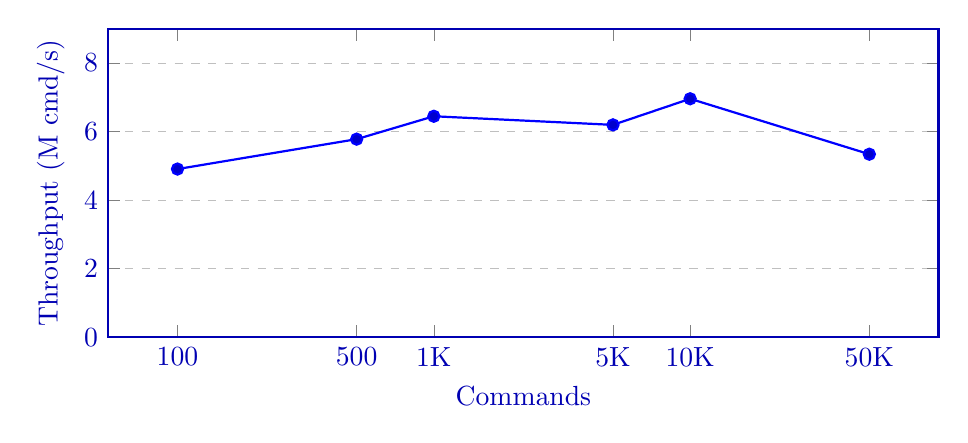
\begin{tikzpicture}
\begin{axis}[
    width=\linewidth, height=5.5cm,
    xlabel={Commands},
    ylabel={Throughput (M cmd/s)},
    xmode=log,
    xtick={100,500,1000,5000,10000,50000},
    xticklabels={100,500,1K,5K,10K,50K},
    ymin=0, ymax=9,
    ymajorgrids=true,
    grid style=dashed,
    mark=*,
    thick,
    color=blue!70!black,
]
\addplot coordinates {
    (100,   4.908)
    (500,   5.780)
    (1000,  6.448)
    (5000,  6.197)
    (10000, 6.958)
    (50000, 5.341)
};
\end{axis}
\end{tikzpicture}
\caption{Replay throughput remains stable at 5–7 M cmd/s regardless of log size.}
\label{fig:throughput}
\end{figure}

During development, this benchmark identified a quadratic performance issue in the initial implementation. The original \texttt{ReplayAll} called \texttt{MarkFlushed} once per resolved command, each of which performed a linear scan of the pending vector. This produced O($n^2$) behaviour: 50,000 commands took 2,939 ms before the fix. The fix — collecting all resolved keys and removing them in a single pass — reduced that to 9 ms, a 313-fold improvement.

\subsection{Command Log Backend Comparison}

The second benchmark compares the in-memory \texttt{CommandLog} against the SQLite-backed \texttt{SQLiteCommandLog} for append and retrieval operations.

\begin{center}
\begin{tabular}{rrrrr}
\hline
Commands & Mem. Append (ms) & SQL Append (ms) & Mem. Get (ms) & SQL Get (ms) \\
\hline
100      & 0.00             & 0.33            & 0.00          & 0.03         \\
1,000    & 0.01             & 3.35            & 0.00          & 0.20         \\
5,000    & 0.06             & 19.96           & 0.02          & 1.06         \\
10,000   & 0.13             & 33.57           & 0.03          & 1.82         \\
\hline
\end{tabular}
\end{center}

SQLite append is approximately 250 times slower than in-memory (33 ms vs 0.13 ms for 10,000 commands), as shown in Figure~\ref{fig:backends}; this is expected given that SQLite writes to disk with ACID guarantees. In absolute terms the overhead is still acceptable for an offline session: a player generating 10,000 actions — far more than a typical session — would incur roughly 33 ms of storage overhead. Retrieval via \texttt{GetPending} is fast in both backends; at 10,000 commands SQLite takes under 2 ms.

\begin{figure}[h]
\centering
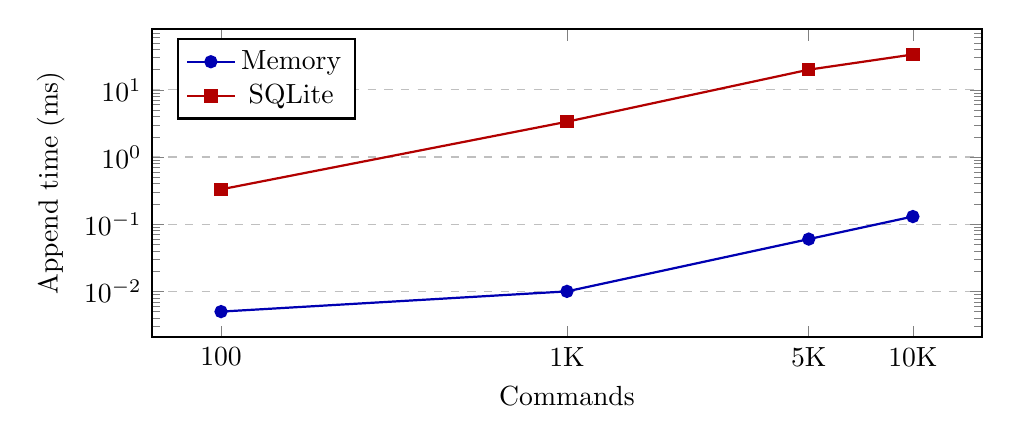
\begin{tikzpicture}
\begin{axis}[
    width=\linewidth, height=5.5cm,
    xlabel={Commands},
    ylabel={Append time (ms)},
    xmode=log,
    ymode=log,
    xtick={100,1000,5000,10000},
    xticklabels={100,1K,5K,10K},
    ymajorgrids=true,
    grid style=dashed,
    legend pos=north west,
    thick,
]
\addplot[color=blue!70!black, mark=*] coordinates {
    (100,  0.005)
    (1000, 0.01)
    (5000, 0.06)
    (10000,0.13)
};
\addlegendentry{Memory}
\addplot[color=red!70!black, mark=square*] coordinates {
    (100,  0.33)
    (1000, 3.35)
    (5000, 19.96)
    (10000,33.57)
};
\addlegendentry{SQLite}
\end{axis}
\end{tikzpicture}
\caption{SQLite append is $\sim$250$\times$ slower than in-memory due to ACID disk writes; both scale linearly.}
\label{fig:backends}
\end{figure}

\subsection{Conflict Detection Overhead}

The third benchmark holds the command count fixed at 10,000 and varies the proportion of commands that are guaranteed to produce a version conflict, from 0\% to 100\%.

\begin{center}
\begin{tabular}{rrrr}
\hline
Conflict rate & Time (ms) & Throughput (cmd/s) & Applied \\
\hline
0\%           & 1.10      & 9,130,686          & 3,246   \\
25\%          & 0.92      & 10,898,185         & 3,213   \\
50\%          & 0.93      & 10,696,617         & 3,175   \\
75\%          & 0.98      & 10,163,025         & 3,085   \\
100\%         & 0.89      & 11,230,176         & 2,912   \\
\hline
\end{tabular}
\end{center}

Throughput varies by less than 20\% across the full range of conflict rates (Figure~\ref{fig:conflicts}). Higher conflict rates are marginally faster because rejected commands skip the database write step. This confirms that the version check and classification logic add negligible overhead and that the system degrades gracefully under adversarial conflict conditions.

\begin{figure}[h]
\centering
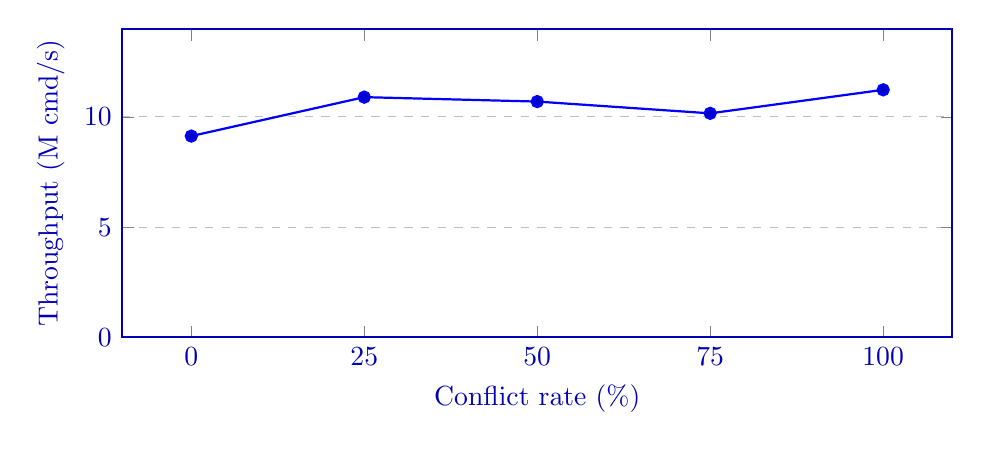
\begin{tikzpicture}
\begin{axis}[
    width=\linewidth, height=5.5cm,
    xlabel={Conflict rate (\%)},
    ylabel={Throughput (M cmd/s)},
    xtick={0,25,50,75,100},
    ymin=0, ymax=14,
    ymajorgrids=true,
    grid style=dashed,
    mark=*,
    thick,
    color=blue!70!black,
]
\addplot coordinates {
    (0,   9.131)
    (25,  10.898)
    (50,  10.697)
    (75,  10.163)
    (100, 11.230)
};
\end{axis}
\end{tikzpicture}
\caption{Throughput remains within 20\% across all conflict rates, confirming conflict detection adds negligible overhead.}
\label{fig:conflicts}
\end{figure}

\subsection{Full Offline Session Round-Trip}

The fourth benchmark measures the complete cost of an offline session using the SQLite command log: appending commands to the durable log, retrieving them, and replaying against the in-memory database.

\begin{center}
\begin{tabular}{rrrrrr}
\hline
Commands & Append (ms) & GetPending (ms) & ReplayAll (ms) & Total (ms) \\
\hline
100      & 0.30        & 0.02            & 0.15           & 0.47       \\
1,000    & 2.86        & 0.17            & 0.81           & 3.84       \\
5,000    & 15.26       & 0.84            & 3.09           & 19.19      \\
10,000   & 30.42       & 1.70            & 6.29           & 38.40      \\
\hline
\end{tabular}
\end{center}

A full session of 10,000 commands completes in approximately 38 ms end-to-end (Figure~\ref{fig:roundtrip}). SQLite append accounts for roughly 80\% of that time; actual replay takes only 6 ms. All three phases scale linearly with command count. The results indicate that reconnection latency attributable to synchronization is unlikely to be noticeable in practice for sessions of realistic size.

\begin{figure}[h]
\centering
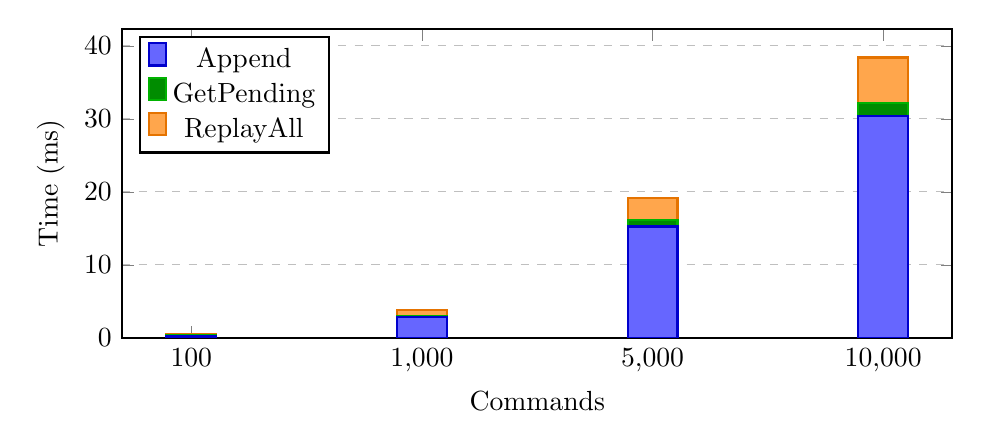
\begin{tikzpicture}
\begin{axis}[
    width=\linewidth, height=5.5cm,
    xlabel={Commands},
    ylabel={Time (ms)},
    ybar stacked,
    bar width=18pt,
    xtick={1,2,3,4},
    xticklabels={100, 1{,}000, 5{,}000, 10{,}000},
    ymin=0,
    ymajorgrids=true,
    grid style=dashed,
    legend style={at={(0.02,0.98)}, anchor=north west},
    thick,
]
\addplot[fill=blue!60, draw=blue!80!black] coordinates {
    (1, 0.30) (2, 2.86) (3, 15.26) (4, 30.42)
};
\addlegendentry{Append}
\addplot[fill=green!55!black, draw=green!70!black] coordinates {
    (1, 0.02) (2, 0.17) (3, 0.84) (4, 1.70)
};
\addlegendentry{GetPending}
\addplot[fill=orange!70, draw=orange!90!black] coordinates {
    (1, 0.15) (2, 0.81) (3, 3.09) (4, 6.29)
};
\addlegendentry{ReplayAll}
\end{axis}
\end{tikzpicture}
\caption{Full offline session cost broken down by phase; SQLite append dominates at $\sim$80\% of total time.}
\label{fig:roundtrip}
\end{figure}

\subsection{Command Log Disk Footprint}

The fifth benchmark measures how much disk space the SQLite-backed command log consumes as a function of log size. Commands are generated with UUID-length idempotency keys (36 characters) to reflect realistic production identifiers. File size is measured after the database connection is closed, including any WAL file that was not checkpointed.

\begin{center}
\begin{tabular}{rrr}
\hline
Commands & File size (KB) & Bytes per command \\
\hline
100      & 32.0           & 327.7 \\
500      & 80.0           & 163.8 \\
1,000    & 140.0          & 143.4 \\
5,000    & 628.0          & 128.6 \\
10,000   & 1,248.0        & 127.8 \\
\hline
\end{tabular}
\end{center}

The per-command cost stabilizes at approximately 128 bytes for logs of 1,000 commands or more. This overhead has two components: the raw data content of each row (idempotency key at 36 bytes, type string at approximately 13 bytes, entity ID, two integers, and timestamp — roughly 75 bytes in total) and SQLite's structural overhead from the B-tree page layout and the secondary index on the \texttt{idempotency\_key} column, which adds approximately 50 bytes per row.

The high per-command cost at small log sizes (327 bytes at 100 commands) is a consequence of SQLite's fixed page size of 4 KB: even a single-row database occupies at least two pages — one for the data table and one for the unique index. Once the log grows large enough to fill pages efficiently the overhead drops to the steady-state figure.

In practical terms, a 1,000-command offline session — already a large session by most standards — occupies 140 KB. A session of 10,000 commands occupies approximately 1.2 MB (Figure~\ref{fig:diskfootprint}). These figures are negligible on any modern storage medium and confirm that disk space is not a limiting factor for the command log approach.

\begin{figure}[h]
\centering
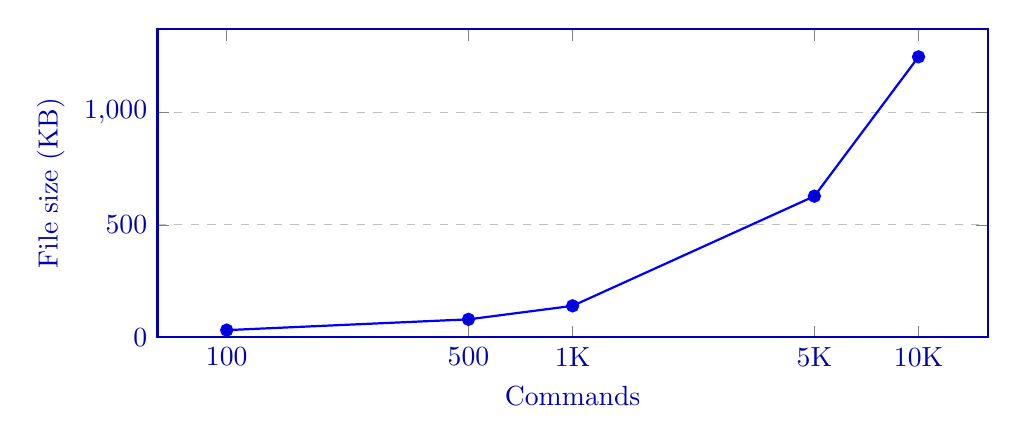
\begin{tikzpicture}
\begin{axis}[
    width=\linewidth, height=5.5cm,
    xlabel={Commands},
    ylabel={File size (KB)},
    xmode=log,
    xtick={100,500,1000,5000,10000},
    xticklabels={100,500,1K,5K,10K},
    ymin=0,
    ymajorgrids=true,
    grid style=dashed,
    mark=*,
    thick,
    color=blue!70!black,
]
\addplot coordinates {
    (100,   32)
    (500,   80)
    (1000,  140)
    (5000,  628)
    (10000, 1248)
};
\end{axis}
\end{tikzpicture}
\caption{Command log file size grows linearly with command count; 10{,}000 commands occupy $\sim$1.2 MB.}
\label{fig:diskfootprint}
\end{figure}

\subsection{Network Latency Model}

All previous benchmarks measure local processing cost in isolation. To place those figures in context, the sixth experiment models the full reconnection time by combining the measured local cost with a simple analytical network overhead. The command log is treated as a single batch request: the client serializes all pending commands, transmits them to the server, and waits for the rejection manifest. Under this model the network contribution to reconnection time is:

\[
t_{\text{network}} = \frac{\text{RTT}}{1 - p_{\text{loss}}}
\]

where RTT is the round-trip time and $p_{\text{loss}}$ is the packet loss rate. The denominator accounts for geometric retransmission: on a lossy link each attempt succeeds with probability $1 - p_{\text{loss}}$, so the expected number of attempts is $1/(1-p_{\text{loss}})$.

Five representative network conditions are tested against three command log sizes.

\begin{center}
\begin{tabular}{lrrrr}
\hline
Network & Commands & Local (ms) & Network (ms) & Total (ms) \\
\hline
No network   & 100   & 0.52  & 0.00   & 0.52   \\
LAN          & 100   & 0.52  & 2.00   & 2.52   \\
Broadband    & 100   & 0.52  & 40.20  & 40.73  \\
Mobile       & 100   & 0.52  & 122.45 & 122.97 \\
Poor mobile  & 100   & 0.52  & 315.79 & 316.31 \\
\hline
No network   & 1,000 & 4.12  & 0.00   & 4.12   \\
LAN          & 1,000 & 4.12  & 2.00   & 6.12   \\
Broadband    & 1,000 & 4.12  & 40.20  & 44.32  \\
Mobile       & 1,000 & 4.12  & 122.45 & 126.57 \\
Poor mobile  & 1,000 & 4.12  & 315.79 & 319.91 \\
\hline
No network   & 10,000 & 40.22 & 0.00   & 40.22  \\
LAN          & 10,000 & 40.22 & 2.00   & 42.22  \\
Broadband    & 10,000 & 40.22 & 40.20  & 80.43  \\
Mobile       & 10,000 & 40.22 & 122.45 & 162.67 \\
Poor mobile  & 10,000 & 40.22 & 315.79 & 356.01 \\
\hline
\end{tabular}
\end{center}

For small logs (100 commands), the local cost is negligible at 0.5 ms; reconnection time is dominated almost entirely by network latency regardless of log size. Even on a poor mobile connection (300 ms RTT, 5\% loss), a 10,000-command log synchronizes in approximately 356 ms — well under half a second for what is already an unrealistically large offline session. Figure~\ref{fig:network} visualises the local–network breakdown for the 10,000-command case.

\begin{figure}[h]
\centering
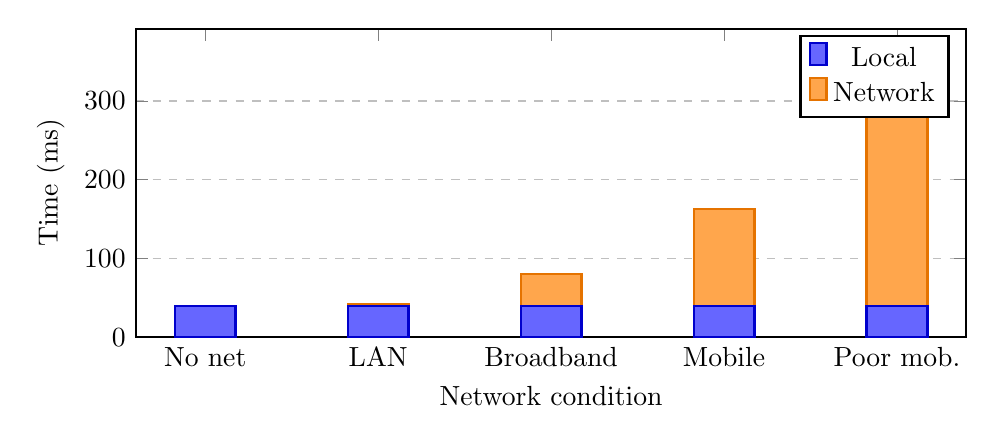
\begin{tikzpicture}
\begin{axis}[
    width=\linewidth, height=5.5cm,
    xlabel={Network condition},
    ylabel={Time (ms)},
    ybar stacked,
    bar width=22pt,
    xtick={1,2,3,4,5},
    xticklabels={No net, LAN, Broadband, Mobile, Poor mob.},
    ymin=0,
    ymajorgrids=true,
    grid style=dashed,
    legend style={at={(0.98,0.98)}, anchor=north east},
    thick,
]
\addplot[fill=blue!60, draw=blue!80!black] coordinates {
    (1,40.22)(2,40.22)(3,40.22)(4,40.22)(5,40.22)
};
\addlegendentry{Local}
\addplot[fill=orange!70, draw=orange!90!black] coordinates {
    (1,0)(2,2.00)(3,40.20)(4,122.45)(5,315.79)
};
\addlegendentry{Network}
\end{axis}
\end{tikzpicture}
\caption{Reconnection time breakdown for 10{,}000 commands: local processing is constant at $\sim$40 ms; network RTT dominates under high-latency conditions.}
\label{fig:network}
\end{figure}

The crossover point — where network overhead equals local processing cost — occurs at approximately 40 ms RTT, which corresponds to a mid-range broadband connection. Below that threshold (LAN), the synchronization mechanism itself is the bottleneck; above it, the network is. This suggests that for real-world deployments the primary lever for reducing reconnection time is reducing the size of the command log (for example, by coalescing commutative deltas) rather than optimising the local replay engine further.

\newpage

\section{Discussion}
\label{sec:discussion}

\subsection{Architectural Trade-offs}

There are many different ways to implement world persistence for online multiplayer games. Each model has its own set of advantages and disadvantages in terms of consistency, flexibility, and complexity.

Offline play becomes impossible with a purely server-authoritative architecture. However, it does provide strong consistency through having a single source of truth. This is because of the CAP theorem \autocite{gilbert2002cap}: consistency, availability, and partition tolerance cannot be accomplished simultaneously, only two of the three are possible at a time. A server-authoritative model focuses on consistency, and will not accept modification to the database if the network is partitioned (i.e. the client is offline). In the hybrid approach, as presented in this thesis, writing to the database is made possible locally while offline (during a partition), and is then later validated on reconnection. Consistency is sacrificed for the sake of availability, conflict resolution is used to restore consistency later on.

This hybrid approach is a middle-ground between an always online model, and always offline architecture. The Command-based model allows offline sessions, known as partitioning, which can later be synchronized and return as an online session. Synchronization does not happen by taking the diffs of two databases and adding them together, instead the suggested approach involves replaying commands which have been logged during the offline play session in the same order in which they are recorded, the intent of the player is preserved. Transactions on the server stay the same, the design doesn't require a major redesign of a typical and preexisting server-authoritative architecture. The greatest difficulty with this approach is to develop systems to recognize conflicts and to validate them on the server. Despite a complicated conflict-resolution implementation, this Command-based persistence method is still less invasive to the existing persistence layer in a server-authoritative architecture compared to adopting Conflict-free Replicated Data Types (CRDT) or the Operational Transformation (OT) approach.

\subsection{Evaluation Findings}

A C++ implementation was developed and benchmark results were made to support the architectural claims in the following ways:

The replay throughput experiments demonstrate that processing a command log of 10.000 has a total time of less than 2 ms in-memory and 38 ms including SQLite retrieval. These values indicate that in practice logging and running synchronization on reconnection will likely result in negligible loading times. This data sent on reconnection is proportional to number of actions performed offline and not the size of the world, in large persistent worlds this will likely be less data compared to snapshot-based methods.

The result of the conflict rate experiment is of particular use: throughput is not much affected by the conflict rate over the entire range of conflict rates, from 0\% to 100\%. This implies that the system does not have a significant degradation in adverse situations and that detection of conflict is not a limiting factor, but rather can be considered as a small overhead.

Even on a bad mobile network (300 ms RTT, 5\% packet loss), the network latency model indicates that a 10.000-command log takes about 356 ms end-to-end to reconnect. If you have a connection speed of, say, below 40 ms RTT, then the processing cost will be the dominant factor, whereas if you have, say, above that, then the network latency will take over. In practice, compacting commutative deltas to save log space is a better optimisation than making replay more responsive for players on high latency connections.

As part of the benchmarking process, the first implementation was found to be flawed. The original \texttt{ReplayAll} was making individual calls to \texttt{MarkFlushed} on each command that was being resolved, all of which did a linear scan on the pending vector. This gave rise to O($n^2$) behaviour: 50.000 commands used almost 3 seconds. This was reduced to 9 ms after a fix. This is one example of the benefits of performance testing, not only as a check at the end of the design process but during development as well.

\subsection{Scalability Considerations}
\label{sec:scale}

The benchmarks characterise the performance of a single-client replay on one machine, which is a necessary but not sufficient basis for scalability claims about a large-scale multiplayer game. Several factors outside the scope of the prototype would affect performance in a production environment.

The server-side validation logic — checking entity versions and preconditions — was evaluated against an in-memory store. Against a real SQL database under concurrent load from many reconnecting players, validation throughput would depend heavily on database indexing, connection pooling, and transaction isolation levels. The benchmarks use a synthetic workload with uniformly distributed entity access. Real player behaviour may be bursty and spatially clustered, which could affect conflict rates and cache behaviour in ways not captured by the synthetic experiments.

These limitations do not undermine the core design, but they do mean that the benchmark results should be treated as indicative of single-client algorithmic performance rather than a prediction of production capacity.

\subsection{Limitations and Threats to Validity}

The conflict resolution strategy handles the three command classes identified in this thesis — idempotent, commutative, and non-commutative — but does not cover all edge cases that a production system would encounter. The most significant gap is commands that depend on entities which were deleted server-side during the offline session: these are caught by the existence check in \texttt{ReplayCommand}, but the player receives only a rejection notification with no automatic recovery path. A production system would need policies for how to surface and resolve these failures in a way that makes sense within the game's design.

The evaluation workload was generated synthetically using a uniform random distribution over entities and command types. It is not known whether this distribution is representative of real player behaviour, which likely varies by game genre, session length, and player experience level. Collecting telemetry from real offline sessions would allow future work to calibrate the benchmark parameters and test the system under more realistic conditions.

Entity versioning relies on an implicit assumption that the server is the sole authority over version increments and that the counter is strictly monotonic. Under these conditions accidental version alignment is not possible: because versions only increase, any server-side modification to an entity will produce a version strictly higher than what the client recorded offline, and the mismatch will be detected correctly. However, this guarantee depends entirely on correct server-side implementation — a bug that modifies an entity without incrementing its version would silently pass the version check, allowing a potentially conflicting command to be committed. An alternative that does not carry this assumption is to store a cryptographic hash of the entity state alongside the version number. Because a hash reflects the actual content of the entity rather than a counter, it detects state changes even if the version increment is accidentally omitted. The trade-off is cost: hashing the full entity state on every command validation is more expensive than an integer comparison, and under reconnection load from many concurrent clients the overhead compounds. For a trusted server-authoritative environment the integer counter is sufficient; the hash approach is better suited to settings where the integrity of the version counter itself cannot be fully guaranteed.

\subsection{Game Preservation}

Beyond the technical design, offline functionality has an important consequence for the long-term availability of games as cultural artefacts. Games that depend on continuous server connectivity cease to function when the developer shuts down the online service, whether due to bankruptcy, acquisition, or commercial decision. Building in offline capability means that the game remains playable independently of the publisher's infrastructure, which is directly relevant to current policy debates around game preservation \autocite{ross}.

\subsection{Financial Considerations}

Offline capability also has practical consequences for both players and developers that extend beyond technical design.

From the player perspective, accessing online multiplayer on console platforms typically requires a paid subscription — PlayStation Plus, Xbox Game Pass Core, or Nintendo Switch Online. An offline-capable design removes this financial barrier \autocite{onlinegamers}, and broadens the reachable audience without requiring any change to the online multiplayer experience for players who do subscribe.

From the developer perspective, running always-on server infrastructure for a large-scale multiplayer game is expensive. Servers must remain provisioned and operational at all times, regardless of how many players are actually connected, to guarantee immediate availability when players log in. A hybrid architecture reduces this pressure: players who are offline generate no server load, and infrastructure can be scaled closer to active concurrent usage rather than peak theoretical demand.

\newpage

\section{Future Work}
\label{sec:futurework}

Several directions for future investigation emerge from the limitations identified in this thesis.

\textbf{Telemetry-calibrated benchmarks.} The evaluation used synthetically generated command logs with uniform random distributions. Collecting real telemetry from offline gameplay sessions would allow the benchmark parameters — entity access distributions, session lengths, conflict rates — to be calibrated against actual player behaviour. This would give a more reliable picture of expected performance and surface corner cases that synthetic workloads may miss.

\textbf{Production server-side scaling.} The server-side replay was evaluated against an in-memory entity store. A production deployment would run validation against a live SQL database under concurrent load from many clients reconnecting simultaneously. Future work should measure how the validation pipeline scales with database contention, test appropriate transaction isolation levels, and explore batching strategies for the server-side replay endpoint.

\textbf{Network latency modelling.} Replay throughput was measured locally, but in practice the command log is transmitted over a network before server-side validation begins. A more complete evaluation would model round-trip latency and measure how command log size affects reconnection time across different network conditions.

\textbf{Recovery paths for rejected commands.} The current design returns a rejection manifest to the client but does not specify what the game should do with it. A production system would need player-facing flows for communicating which offline actions were declined and offering resolution options — for example, refunding consumed resources or offering equivalent substitute items. Designing these recovery policies in a way that is both technically correct and satisfying to players is a non-trivial game-design problem.

\textbf{Command dependency graphs.} Some commands may depend on earlier commands in the same offline log — for example, building a structure and then upgrading it. If the first command is rejected, the second is also invalid regardless of its version check. Modelling explicit command dependencies would allow the replay engine to reject dependent chains early and produce more informative rejection manifests.

\newpage

\section{Conclusion}
\label{sec:conclusion}

This thesis investigated the following research question: How can an offline-online synchronization system for game persistence targeting survival multiplayer games be designed and evaluated with respect to consistency, conflict resolution, and reconnection performance?

The starting point was a server-authoritative persistence architecture in which all state changes are executed as transactional SQL operations against a centralized cloud backend. While robust in fully online environments, this model assumes continuous connectivity and does not support offline progression or hybrid play modes. Enabling offline functionality therefore requires architectural changes that preserve data integrity while allowing temporary divergence of state.

Two alternative approaches were evaluated before arriving at the proposed design. Direct local database mirroring through SQLite provides a familiar persistence interface during offline sessions but does not itself address how divergent state is reconciled upon reconnection. An object–relational mapping layer was also considered but rejected due to a fundamental mismatch: an ORM tracks object state rather than operations, which is incompatible with the command-based replication model.

The proposed solution is a command-based replication model. Rather than synchronizing complete world snapshots, the system records player intent as serializable commands that can be replayed deterministically against the authoritative server. This approach addresses the three dimensions of the research question as follows.

\textbf{Consistency} is maintained by treating the cloud server as the single authoritative source of truth. Offline commands are not committed until they have been validated and replayed server-side. The transactional guarantees of the SQL backend are preserved throughout.

\textbf{Conflict resolution} is handled through a combination of entity versioning, command classification, and per-type resolution policies. Idempotent commands are replayed unconditionally; commutative operations such as resource deltas are merged by summation; and non-commutative operations are validated against current server state before being accepted or rejected. Commands that cannot be applied are returned to the client in a rejection manifest rather than being silently discarded.

\textbf{Reconnection performance} was evaluated through a suite of benchmarks on a single development machine, including a network latency model. A log of 10,000 commands replays in under 2 ms in memory and under 40 ms end-to-end including SQLite persistence. When network overhead is added, even a poor mobile connection (300 ms RTT, 5\% packet loss) produces a total reconnection time of approximately 356 ms. Conflict detection adds less than 20\% overhead regardless of conflict rate, and the command log file remains under 1.2 MB at 10,000 commands. These results indicate that the synchronization mechanism itself is unlikely to be a perceptible bottleneck during reconnection for sessions of realistic size.

The approach introduces its own requirements: commands must be deterministic and replay-safe, ordering must be preserved across the command log, and server-side validation logic must cover all command types to prevent exploitation. These constraints are manageable within a server-authoritative architecture but would require careful engineering in a production system.

Overall, the results suggest that a command-based synchronization model provides a practical and extensible foundation for hybrid offline–online persistence in survival video games, and that consistent synchronization can be achieved without fundamentally redesigning a server-authoritative framework.

\newpage

\glsaddall
\printglossaries

\newpage

\printbibliography

\end{document}
